\subsection{Cost estimation Evaluation} \label{CostsExper}
In this section we present the results of using different cost estimation methods discussed
previously Actual Costs and DB estimates.
%\mas{so cost was not used in the previous set of experiments?!}

In our experiments we used GoCard dataset which is Brisbane transportation dataset 
with 4.4 million transactions and it consists of 9 dimension attributes and 3 measures attributes
we run this experiment on SeeDB 
over \emph{All} aggregate functions \emph{Count, Sum, Average, Min, and Max} with 
a space size=$5 \times 9 \times 3=135$ views and 
the deviation metric is Earth Movers Distance (EMD).\\

\footnotesize {$Q:$ Select * from gocard where alightingstop ='University of Queensland'} 

%\thefontsize 
\normalsize  
%\mas{what queries are used for input?}
We are interested in evaluating 
the results of cost estimation methods based on the classical effectiveness and 
efficiency. For effectiveness, we asses the quality of views outputs from the proposed prioritizing 
algorithms $Diff_DVal$, $Sela$, and $DimsHisto$ along different cost estimation methods 
(e.g. DB estimate and Actual Costs) comparing with SeeDB baseline. 
we implemented two baselines strategies: SeeDB baseline which is processes the entire data and evaluates all any views without any cost considerations It thus provides an upper bound on latency and accuracy and lower bound on error distance. The other baseline strategy Actual Costs that computes the actual executions times of all views in addition the actual computational time for measuring the deviation among views.
We measure the quality of results based on the accuracy and error distance measures discussed 
in section. However, the efficiency of estimating methods is captured by rivaling the execution times across proposed prioritizing algorithms  $Diff_DVal$, $Sela$, and $DimsHisto$.
The first experiment is considering to evaluate the results of $Top(25)$ views 
using DB Estimates (reading the costs from database optimizer)
along different space limits while considering the estimated costs of the recommended views compared with the original SeeDB baseline.

In figure \ref{fig:figCost11} shows the accuracy of the results produced by
algorithms $Sela$ , $Diff_DVal$, and $DimHisto$ while reading the costs of the recommended views (queries) from database optimizer to find a top $(K=25)$ views
 along varying view space sizes as shown all algorithms $Sela$ , $Diff_DVal$, and $DimHisto$
  scored about 100\% accuracy starting from  space limit 60 views. 
 % \mas{if the constraint is on the number of views, then why cost is included in the priority?!!! it does not matter if a view takes a second or hour, in the end it counts as one!!}. 
 As 
presented $Sela$ algorithm is the highest accuracy 
%\mas{so why is it the highest now? (compared to previous experiments)} 
and the lowest error distance among all 
proposed algorithms as shown in figure \ref{fig:figCost12}.However, 
in the first views limits 30 and 45 the accuracy of $Diff_DVal$ is very low because it scores views 
only according the difference of distinct values and doesn't consider query size such as $Sela$ %\mas{and why it is very low now?} 
and consequently the error distance is the higher than $Sela$ and $DimsHisto$.
 
% \begin{figure}[h]
%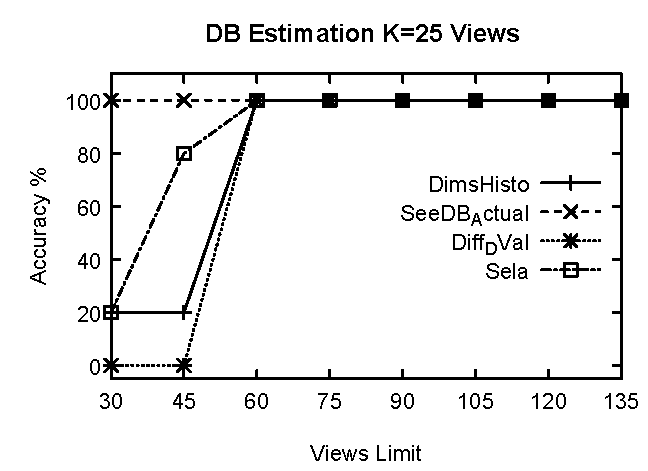
\includegraphics[width=\textwidth]{Cost11.pdf}
%\caption{Accuracy and Error Distance of algorithms $Sela$ , $N-N'$, and $DimsHisto$ across view space limits using DB Estimation}
%\label{fig:figCost11}%
%\end{figure}

\begin{figure}
  \begin{subfigure}[b]{0.45\textwidth}
    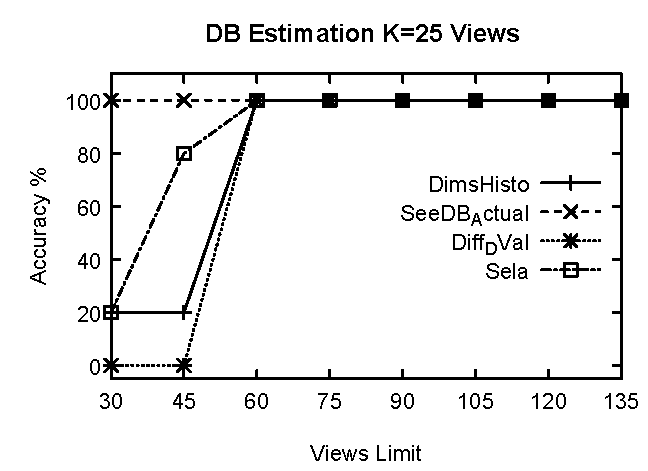
\includegraphics[width=\textwidth]{Cost11.pdf}
    \caption{Accuracy }
    \label{fig:figCost11}%
  \end{subfigure}
  %
  \begin{subfigure}[b]{0.45\textwidth}
    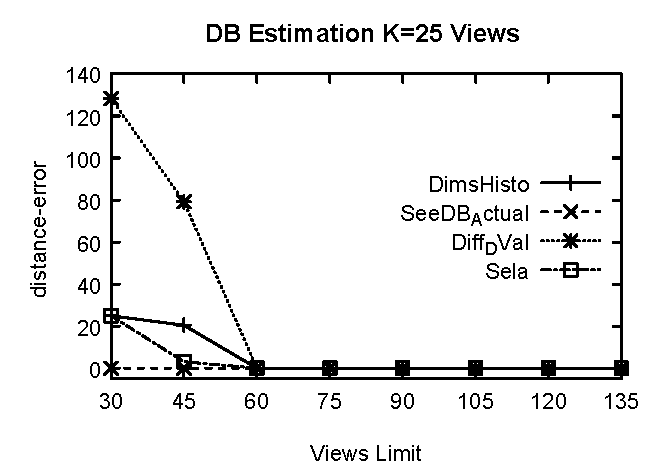
\includegraphics[width=\textwidth]{Cost12.pdf}
  \caption{Distance Error  }
     \label{fig:figCost12}%
  \end{subfigure}
  \caption{ Results quality using DB Estimation  }
  \end{figure}

%\\ In figure \ref{fig:figCost12} shows the accuracy and distance error \mas{No it does not!} of the results produced by
%algorithms $Sela$ , $Diff_DVal$, and $DimHisto$ to find a top $(K=25)$ views
 %across different view space sizes using proposed cost model. 
 %As shown algorithm $N-N'$ scored the highest distance error and the 
 %lowest accuracy among all algorithms and the distance error remains high while 
 %extending the space limits. However, $Sela$ shows the best performance 
 %for both accuracy and distance error. $DimHisto$ shows a moderate behaviour 
 %for accuracy and distance error measures but the distance error stable between 
 %space limits 45 and 75 views.
 
%\begin{figure}[h]
%\includegraphics[width=\textwidth]{{Cost12.pdf}}
%\caption{Accuracy and Error Distance of algorithms $Sela$ , $N-N'$, and $DimsHisto$ 
%across view space limits using Cost Model Estimation}
%\label{fig:fig2}%
%\end{figure}

%\\ To sum up, DB Estimate methods shows right estimates of queries than the 
%proposed cost model however, algorithm $Diff_DVal$ showed lower quality than other 
 %proposed algorithms $Sela$ and $DimsHisto$.
  
  The following experiments illustrate the overhead of using different cost 
  estimations techniques along our prioritizing algorithms $Sela$ , $Diff_DVal$, and $DimsHisto$  
  added to the actual SeeDB baseline.
  \begin{figure}
	\centering
 	 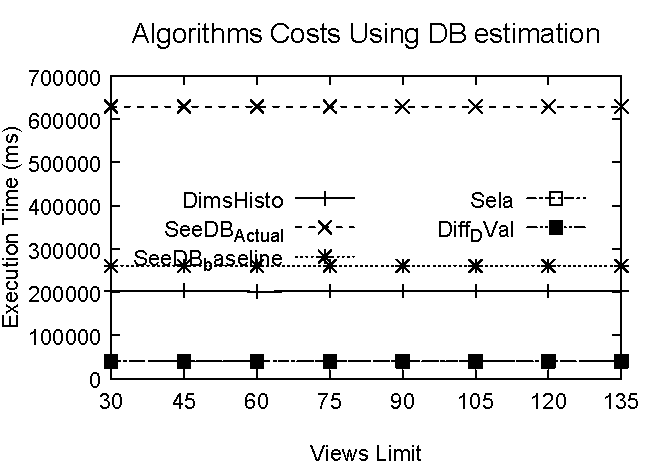
\includegraphics[width=.8\textwidth]{Cost21.pdf}
		 	\caption{Overhead of algorithms using DB Estimation}
	\label{fig:figCost12}
  \end{figure}


  
%  \begin{figure}[h]
%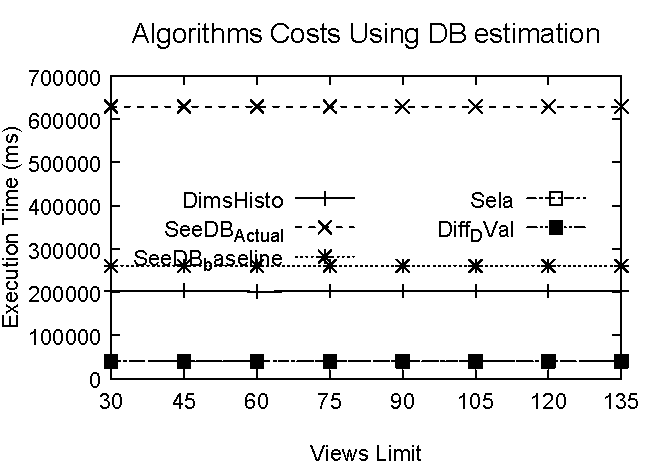
\includegraphics[width=\textwidth]{Cost21.pdf}
%\caption{The overhead of the Algorithms $Sela$ , $N-N'$, and $DimsHisto$ of using DB estimate}
%\label{fig:figCost12}%
%\end{figure}

%\mas{those stacked bars do not make any sense! use some other readable charting}

%\mas{what is the green? blue? so in the end estimate and approx are the same cost?!! those plots are really confusing: 

%use simple intuitive plots 

%be clear about the meaning of the legends: things like SeeDB Actual, SeeDB baseline, Sela Algo Approx are not easy to understand and you did not explain what does it mean! Besides, it is definitely not clear why do you sum them all in one bar!!!}



In Figure \ref{fig:figCost12} shows the overhead of implementing the 
algorithms $Sela$ ,  $Diff_DVal$, and $DimsHisto$ and reading the costs from database
optimizer across different space limits. As shown in figure 
\ref{fig:figCost12}, computing actual costs is much expensive than running SeeDB 
itself this because, SeeDB doesn't execute all aggregate queries for example, the Average 
function of a view is computed by dividing the total values (Sum Aggregate) on their frequency 
(Count Aggregate) moreover, SeeDB combines the aggregate queries of the datasets 
$D$ and $DQ$. All algorithms have a stable performance on different space limits
because the algorithms evaluating the same set of dimension attributes $A$ and outputs
a subset $A'$ of top dimension attributes. As shown, $DimsHisto$ algorithm shows a 
considerable time cost as results of creating and assessing the produced histograms however, both  
algorithms $Sela$ and $Diff_DVal$ have nearly equal execution costs. \\
  
%\begin{figure}[t]
%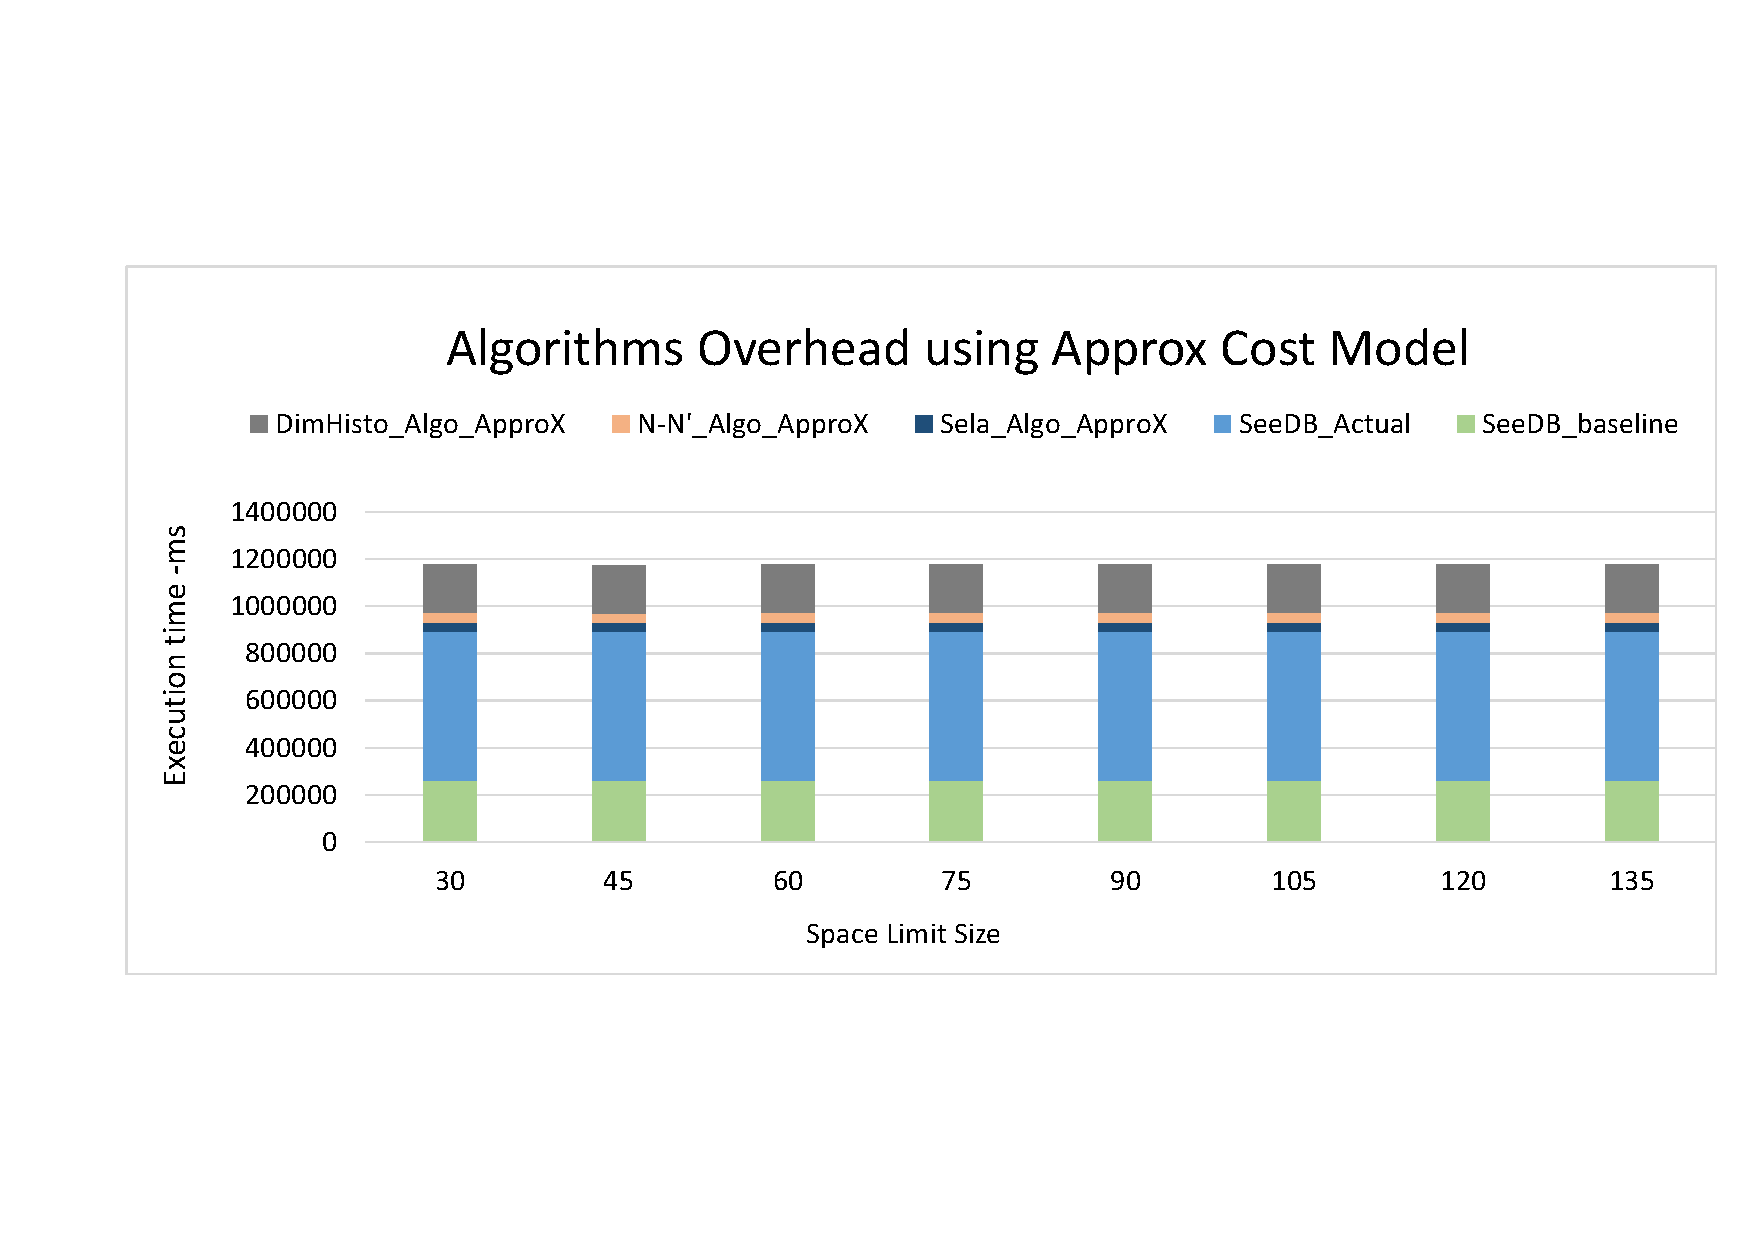
\includegraphics[width=\textwidth]{Cost22.pdf}
%\caption{The overhead of the Algorithms $Sela$ , $N-N'$, and $DimsHisto$ of using Cost Model Estimation}
%\label{fig:figCost22}%
%\end{figure}


In figure \ref{fig:figCost12} shows almost the same performance in the execution times 
as shown in figure \ref{fig:figCost12} along different algorithms $Sela$ , $Diff_DVal$ and 
$DimsHisto$.\\

 In conclusion, the discussed algorithms $Sela$ , $Diff_DVal$, $DimsHisto$ show high 
 accuracy and low distance errors along different space sizes while considering the costs of 
 running and computing the deviation among the corresponding visualizations. we discussed both 
 the results quality and the overhead of running different cost estimation techniques  
 however, our estimation approach can use any I/O cost estimation technique. %\mas{what does that mean?}. 
  